\documentclass[12pt]{article}
\usepackage[english]{babel}
\usepackage[utf8x]{inputenc}
\usepackage[T1]{fontenc}
\usepackage{scribe}
\usepackage{listings}
\usepackage{graphics, graphicx}
\usepackage{enumitem}
\usepackage{tcolorbox}
\usepackage{adjustbox}
\usepackage{algorithm}
\usepackage[english]{babel}
\usepackage{amsthm}
\usepackage[noend]{algpseudocode}
\usepackage{tikz}
\usepackage{forest}
\forestset{
	sn edges1/.style={for tree={edge={->},where n children=0{tier=word}{}}}, 
	background tree/.style={for tree={text opacity=0.2,draw opacity=0.2,edge={draw opacity=0.2}}},
	sn edges2/.style={for tree={edge={<-},where n children=0{tier=word}{}}},
}

\graphicspath{ {./images/} }


\CourseName{Comtemporary Algorithms T.II/2019-20}
\Scribe{Kriangsak T. \& Apivich H.}
\Lecturer{Dr. Kanat Tangwongsan}
\LectureNumber{8}
\LectureDate{29 January 2020}
\LectureTitle{Parallel Algorithms II}

\lstset{style=mystyle}

\newlist{steps}{enumerate}{1}
\setlist[steps, 1]{label = Step \arabic*:}

\algblock{ParFor}{EndParFor}
\algnewcommand\algorithmicparfor{\textbf{parfor}}
\algnewcommand\algorithmicpardo{\textbf{do}}
\algnewcommand\algorithmicendparfor{\textbf{end\ parfor}}
\algrenewtext{ParFor}[2]{\algorithmicparfor\ #1\ \textbf{in}\ #2 \algorithmicpardo}
\algrenewtext{EndParFor}{\algorithmicendparfor}

\tikzset{every picture/.style={line width=0.75pt}} %set default line width to 0.75pt      

\begin{document}
\MakeScribeTop

\section{The Scan Problem}

In the scan problem, we will deal with binary operators $\oplus$ which have associative properties. These are operators which will give the same answer regardless of the order in which the operations are performed in, i.e. $a\oplus (b \oplus c) = (a \oplus b) \oplus c$. Example of such operations are the addition and multiplication of numbers, matrix multiplication, string concatenation, or greatest common divisor operations.

For these operators, we can also define the identity element $e$, such that $x \oplus e = x$ for any $x$ that the operator can be applied on. As an example, for multiplication, its identity element is 1, while for addition, its identity element is 0.

In this section, we will derive a parallel algorithm \textsc{scan($\oplus, e,A = [A[0], A[1], \ldots, A[n-1]]$)} which will return $(S, \Sigma)$, where
\begin{itemize}
	\item $S = [ e, e \oplus A[0], e \oplus A[0] \oplus A[1], \ldots, e \oplus A[0], e \oplus A[0] \oplus \cdots \oplus A[n-3] \oplus A[n-2] ]$, and
	\item $\Sigma = e \oplus A[0] \oplus \cdots \oplus A[n-2] \oplus A[n-1]$.
\end{itemize}
To solve this problem naively, we can just for loop over each elements and add each answer we find to a new array. This would take $O(n)$ work and span (since it has nothing running in parallel whatsoever). We will present a couple of algorithms which improve upon the span of the naive algorithm (since the work cannot be improved upon anyway).

\subsection{Divide-and-Conquer}

The first idea is to use some sort of a divide-and-conquer algorithm. We can divide $A$ into the left half and the right half, and recursively call on the same function on the two halves, then combine the answers. The problem with this, however, is that the answers that we get from the right half will depend on the answers on the left half, and so cannot be done in parallel. 

However, we can get around this by still doing the halves separately, and then combining the answers in a smarter way.
\begin{algorithm}[H]
	\caption{Scan algorithm using divide-and-conquer}
	\label{scdc}
	\begin{algorithmic}[1]
		\Function{ScanDC}{$\oplus, e, A$}
		\State {some base case for recursion}
		\State {$mid \gets |A|/2$}
		\State {$L, R \gets A[:mid], A[mid:]$}
		\State {$(L_p, t_L), (R_p, t_R) \gets \textsc{ScanDC}(\oplus, e, L) \parallel \textsc{ScanDC}(\oplus, e, R)$}
		\ParFor{$i$}{$0,\ldots,|R_p|$}
			\State { $R_p[i] \gets R_p[i] \oplus t_L$ }
		\EndParFor
		\State \Return {$(L_p + R_p, t_L \oplus t_R)$}
		\EndFunction
	\end{algorithmic}
\end{algorithm}
We can show that for an array of size $n$, the work done by the algorithm follows the recursive formula $$W(n) = \underbrace{2W(n/2) }_{\text{Line 5} }+ \underbrace{O(n)}_{\text{Loop in Line 6}}$$ which results in $O(n\lg n)$ overall work, while the span follows the recursive formula $$S(n) = \underbrace{S(n/2) }_{\text{Line 5} } + O(1)$$ which results in $O(\lg n)$ overall span. We can see that while the span has gone down, the work done is now higher than in the naive algorithm, which isn't good. Let's look at another method.

\subsection{Contraction}

Let's look at a concrete example. Suppose we have an array
$$A = [1, 2, 3, 4, 5, 6, 7, 8]$$
and the $\oplus$ operator is just an addition operator. It would be much easier if we instead have an array
$$A' = [3, 7, 11, 15]$$
simply because it's much shorter. Note that $A'$ is just a reduced version of $A$, where every two elements in $A$ is added together. We can call \textsc{Scan} on the smaller array and get
$$\textsc{Scan}(+, 0, A') = ([0, 3, 10, 21], 36)$$
and somehow use this to come up with a final answer. This idea is summarised in the diagram below.

\begin{center}
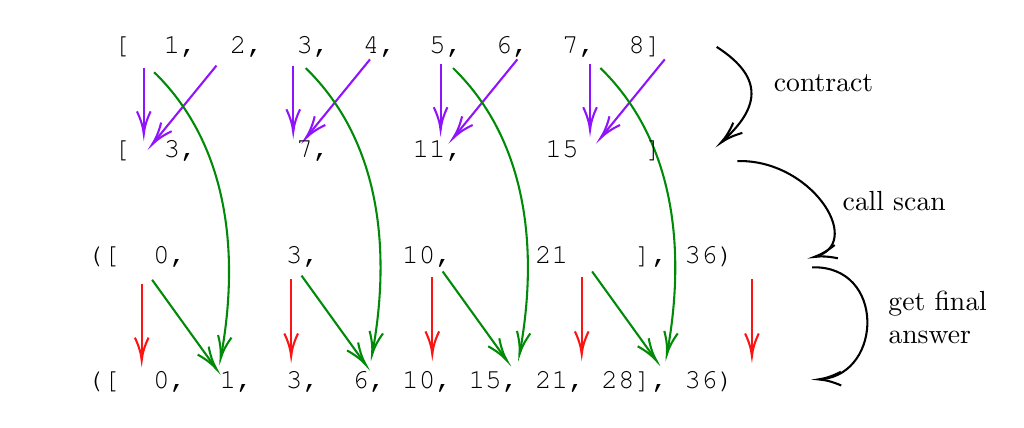
\begin{tikzpicture}[x=0.75pt,y=0.75pt,yscale=-1,xscale=1][c]
%uncomment if require: \path (0,465.8125); %set diagram left start at 0, and has height of 465.8125

%Curve Lines [id:da9944347331385202] 
\draw    (468.5,71.81) .. controls (492.88,87.41) and (487.78,102.24) .. (471.75,116.87) ;
\draw [shift={(470.5,118)}, rotate = 318.58000000000004] [color={rgb, 255:red, 0; green, 0; blue, 0 }  ][line width=0.75]    (10.93,-3.29) .. controls (6.95,-1.4) and (3.31,-0.3) .. (0,0) .. controls (3.31,0.3) and (6.95,1.4) .. (10.93,3.29)   ;

%Curve Lines [id:da062000653304538744] 
\draw    (478.5,126.81) .. controls (513.6,125.84) and (539.19,164.97) .. (517.28,172.49) ;
\draw [shift={(515.5,173)}, rotate = 346.5] [color={rgb, 255:red, 0; green, 0; blue, 0 }  ][line width=0.75]    (10.93,-3.29) .. controls (6.95,-1.4) and (3.31,-0.3) .. (0,0) .. controls (3.31,0.3) and (6.95,1.4) .. (10.93,3.29)   ;

%Curve Lines [id:da4053511849741225] 
\draw    (514.5,178) .. controls (549.78,177.02) and (548.56,228.86) .. (519.33,231.88) ;
\draw [shift={(517.5,232)}, rotate = 358.15] [color={rgb, 255:red, 0; green, 0; blue, 0 }  ][line width=0.75]    (10.93,-3.29) .. controls (6.95,-1.4) and (3.31,-0.3) .. (0,0) .. controls (3.31,0.3) and (6.95,1.4) .. (10.93,3.29)   ;

%Straight Lines [id:da6769829464885964] 
\draw [color={rgb, 255:red, 144; green, 19; blue, 254 }  ,draw opacity=1 ]   (192.5,81.81) -- (192.5,111.81) ;
\draw [shift={(192.5,113.81)}, rotate = 270] [color={rgb, 255:red, 144; green, 19; blue, 254 }  ,draw opacity=1 ][line width=0.75]    (10.93,-3.29) .. controls (6.95,-1.4) and (3.31,-0.3) .. (0,0) .. controls (3.31,0.3) and (6.95,1.4) .. (10.93,3.29)   ;

%Straight Lines [id:da22979436046059476] 
\draw [color={rgb, 255:red, 144; green, 19; blue, 254 }  ,draw opacity=1 ]   (227.5,80.81) -- (197.76,117.26) ;
\draw [shift={(196.5,118.81)}, rotate = 309.21000000000004] [color={rgb, 255:red, 144; green, 19; blue, 254 }  ,draw opacity=1 ][line width=0.75]    (10.93,-3.29) .. controls (6.95,-1.4) and (3.31,-0.3) .. (0,0) .. controls (3.31,0.3) and (6.95,1.4) .. (10.93,3.29)   ;

%Straight Lines [id:da25081808514449544] 
\draw [color={rgb, 255:red, 144; green, 19; blue, 254 }  ,draw opacity=1 ]   (264.5,80.81) -- (264.5,110.81) ;
\draw [shift={(264.5,112.81)}, rotate = 270] [color={rgb, 255:red, 144; green, 19; blue, 254 }  ,draw opacity=1 ][line width=0.75]    (10.93,-3.29) .. controls (6.95,-1.4) and (3.31,-0.3) .. (0,0) .. controls (3.31,0.3) and (6.95,1.4) .. (10.93,3.29)   ;

%Straight Lines [id:da8977084882448785] 
\draw [color={rgb, 255:red, 144; green, 19; blue, 254 }  ,draw opacity=1 ]   (335.5,79.81) -- (335.5,109.81) ;
\draw [shift={(335.5,111.81)}, rotate = 270] [color={rgb, 255:red, 144; green, 19; blue, 254 }  ,draw opacity=1 ][line width=0.75]    (10.93,-3.29) .. controls (6.95,-1.4) and (3.31,-0.3) .. (0,0) .. controls (3.31,0.3) and (6.95,1.4) .. (10.93,3.29)   ;

%Straight Lines [id:da9975595262460375] 
\draw [color={rgb, 255:red, 144; green, 19; blue, 254 }  ,draw opacity=1 ]   (407.5,79.81) -- (407.5,109.81) ;
\draw [shift={(407.5,111.81)}, rotate = 270] [color={rgb, 255:red, 144; green, 19; blue, 254 }  ,draw opacity=1 ][line width=0.75]    (10.93,-3.29) .. controls (6.95,-1.4) and (3.31,-0.3) .. (0,0) .. controls (3.31,0.3) and (6.95,1.4) .. (10.93,3.29)   ;

%Straight Lines [id:da27330516572334185] 
\draw [color={rgb, 255:red, 144; green, 19; blue, 254 }  ,draw opacity=1 ]   (301.5,77.81) -- (271.76,114.26) ;
\draw [shift={(270.5,115.81)}, rotate = 309.21000000000004] [color={rgb, 255:red, 144; green, 19; blue, 254 }  ,draw opacity=1 ][line width=0.75]    (10.93,-3.29) .. controls (6.95,-1.4) and (3.31,-0.3) .. (0,0) .. controls (3.31,0.3) and (6.95,1.4) .. (10.93,3.29)   ;

%Straight Lines [id:da9743754833771201] 
\draw [color={rgb, 255:red, 144; green, 19; blue, 254 }  ,draw opacity=1 ]   (372.5,77.81) -- (342.76,114.26) ;
\draw [shift={(341.5,115.81)}, rotate = 309.21000000000004] [color={rgb, 255:red, 144; green, 19; blue, 254 }  ,draw opacity=1 ][line width=0.75]    (10.93,-3.29) .. controls (6.95,-1.4) and (3.31,-0.3) .. (0,0) .. controls (3.31,0.3) and (6.95,1.4) .. (10.93,3.29)   ;

%Straight Lines [id:da487517695775177] 
\draw [color={rgb, 255:red, 144; green, 19; blue, 254 }  ,draw opacity=1 ]   (443.5,77.81) -- (413.76,114.26) ;
\draw [shift={(412.5,115.81)}, rotate = 309.21000000000004] [color={rgb, 255:red, 144; green, 19; blue, 254 }  ,draw opacity=1 ][line width=0.75]    (10.93,-3.29) .. controls (6.95,-1.4) and (3.31,-0.3) .. (0,0) .. controls (3.31,0.3) and (6.95,1.4) .. (10.93,3.29)   ;

%Straight Lines [id:da5078942772386552] 
\draw [color={rgb, 255:red, 254; green, 19; blue, 19 }  ,draw opacity=1 ]   (191.5,185.81) -- (191.5,220.81) ;
\draw [shift={(191.5,222.81)}, rotate = 270] [color={rgb, 255:red, 254; green, 19; blue, 19 }  ,draw opacity=1 ][line width=0.75]    (10.93,-3.29) .. controls (6.95,-1.4) and (3.31,-0.3) .. (0,0) .. controls (3.31,0.3) and (6.95,1.4) .. (10.93,3.29)   ;

%Straight Lines [id:da24679190993218536] 
\draw [color={rgb, 255:red, 254; green, 19; blue, 19 }  ,draw opacity=1 ]   (263.5,183.81) -- (263.5,218.81) ;
\draw [shift={(263.5,220.81)}, rotate = 270] [color={rgb, 255:red, 254; green, 19; blue, 19 }  ,draw opacity=1 ][line width=0.75]    (10.93,-3.29) .. controls (6.95,-1.4) and (3.31,-0.3) .. (0,0) .. controls (3.31,0.3) and (6.95,1.4) .. (10.93,3.29)   ;

%Straight Lines [id:da9260805821310587] 
\draw [color={rgb, 255:red, 254; green, 19; blue, 19 }  ,draw opacity=1 ]   (331.5,182.81) -- (331.5,217.81) ;
\draw [shift={(331.5,219.81)}, rotate = 270] [color={rgb, 255:red, 254; green, 19; blue, 19 }  ,draw opacity=1 ][line width=0.75]    (10.93,-3.29) .. controls (6.95,-1.4) and (3.31,-0.3) .. (0,0) .. controls (3.31,0.3) and (6.95,1.4) .. (10.93,3.29)   ;

%Straight Lines [id:da3676804982928621] 
\draw [color={rgb, 255:red, 254; green, 19; blue, 19 }  ,draw opacity=1 ]   (403.5,182.81) -- (403.5,217.81) ;
\draw [shift={(403.5,219.81)}, rotate = 270] [color={rgb, 255:red, 254; green, 19; blue, 19 }  ,draw opacity=1 ][line width=0.75]    (10.93,-3.29) .. controls (6.95,-1.4) and (3.31,-0.3) .. (0,0) .. controls (3.31,0.3) and (6.95,1.4) .. (10.93,3.29)   ;

%Straight Lines [id:da21841617521729995] 
\draw [color={rgb, 255:red, 1; green, 138; blue, 7 }  ,draw opacity=1 ]   (196.5,184) -- (226.33,225.38) ;
\draw [shift={(227.5,227)}, rotate = 234.21] [color={rgb, 255:red, 1; green, 138; blue, 7 }  ,draw opacity=1 ][line width=0.75]    (10.93,-3.29) .. controls (6.95,-1.4) and (3.31,-0.3) .. (0,0) .. controls (3.31,0.3) and (6.95,1.4) .. (10.93,3.29)   ;

%Straight Lines [id:da24386663118770846] 
\draw [color={rgb, 255:red, 1; green, 138; blue, 7 }  ,draw opacity=1 ]   (268.5,182) -- (298.33,223.38) ;
\draw [shift={(299.5,225)}, rotate = 234.21] [color={rgb, 255:red, 1; green, 138; blue, 7 }  ,draw opacity=1 ][line width=0.75]    (10.93,-3.29) .. controls (6.95,-1.4) and (3.31,-0.3) .. (0,0) .. controls (3.31,0.3) and (6.95,1.4) .. (10.93,3.29)   ;

%Straight Lines [id:da20300387958362198] 
\draw [color={rgb, 255:red, 1; green, 138; blue, 7 }  ,draw opacity=1 ]   (336.5,180) -- (366.33,221.38) ;
\draw [shift={(367.5,223)}, rotate = 234.21] [color={rgb, 255:red, 1; green, 138; blue, 7 }  ,draw opacity=1 ][line width=0.75]    (10.93,-3.29) .. controls (6.95,-1.4) and (3.31,-0.3) .. (0,0) .. controls (3.31,0.3) and (6.95,1.4) .. (10.93,3.29)   ;

%Straight Lines [id:da7792356175625177] 
\draw [color={rgb, 255:red, 1; green, 138; blue, 7 }  ,draw opacity=1 ]   (408.5,180) -- (438.33,221.38) ;
\draw [shift={(439.5,223)}, rotate = 234.21] [color={rgb, 255:red, 1; green, 138; blue, 7 }  ,draw opacity=1 ][line width=0.75]    (10.93,-3.29) .. controls (6.95,-1.4) and (3.31,-0.3) .. (0,0) .. controls (3.31,0.3) and (6.95,1.4) .. (10.93,3.29)   ;

%Straight Lines [id:da7267253542639487] 
\draw [color={rgb, 255:red, 254; green, 19; blue, 19 }  ,draw opacity=1 ]   (485.5,183.81) -- (485.5,218.81) ;
\draw [shift={(485.5,220.81)}, rotate = 270] [color={rgb, 255:red, 254; green, 19; blue, 19 }  ,draw opacity=1 ][line width=0.75]    (10.93,-3.29) .. controls (6.95,-1.4) and (3.31,-0.3) .. (0,0) .. controls (3.31,0.3) and (6.95,1.4) .. (10.93,3.29)   ;

%Curve Lines [id:da48346921848254065] 
\draw [color={rgb, 255:red, 1; green, 138; blue, 7 }  ,draw opacity=1 ]   (197.5,84) .. controls (234.13,119.64) and (238.42,172.92) .. (229.77,220.56) ;
\draw [shift={(229.5,222)}, rotate = 280.62] [color={rgb, 255:red, 1; green, 138; blue, 7 }  ,draw opacity=1 ][line width=0.75]    (10.93,-3.29) .. controls (6.95,-1.4) and (3.31,-0.3) .. (0,0) .. controls (3.31,0.3) and (6.95,1.4) .. (10.93,3.29)   ;

%Curve Lines [id:da28400465711081346] 
\draw [color={rgb, 255:red, 1; green, 138; blue, 7 }  ,draw opacity=1 ]   (270.5,82) .. controls (307.13,117.64) and (311.42,170.92) .. (302.77,218.56) ;
\draw [shift={(302.5,220)}, rotate = 280.62] [color={rgb, 255:red, 1; green, 138; blue, 7 }  ,draw opacity=1 ][line width=0.75]    (10.93,-3.29) .. controls (6.95,-1.4) and (3.31,-0.3) .. (0,0) .. controls (3.31,0.3) and (6.95,1.4) .. (10.93,3.29)   ;

%Curve Lines [id:da05174392639065606] 
\draw [color={rgb, 255:red, 1; green, 138; blue, 7 }  ,draw opacity=1 ]   (341.5,82) .. controls (378.13,117.64) and (382.42,170.92) .. (373.77,218.56) ;
\draw [shift={(373.5,220)}, rotate = 280.62] [color={rgb, 255:red, 1; green, 138; blue, 7 }  ,draw opacity=1 ][line width=0.75]    (10.93,-3.29) .. controls (6.95,-1.4) and (3.31,-0.3) .. (0,0) .. controls (3.31,0.3) and (6.95,1.4) .. (10.93,3.29)   ;

%Curve Lines [id:da8566555089886099] 
\draw [color={rgb, 255:red, 1; green, 138; blue, 7 }  ,draw opacity=1 ]   (412.5,82) .. controls (449.13,117.64) and (453.42,170.92) .. (444.77,218.56) ;
\draw [shift={(444.5,220)}, rotate = 280.62] [color={rgb, 255:red, 1; green, 138; blue, 7 }  ,draw opacity=1 ][line width=0.75]    (10.93,-3.29) .. controls (6.95,-1.4) and (3.31,-0.3) .. (0,0) .. controls (3.31,0.3) and (6.95,1.4) .. (10.93,3.29)   ;


% Text Node
\draw (310,71.81) node   [align=left] {{\fontfamily{pcr}\selectfont [ \ 1, \ 2, \ 3, \ 4, \ 5, \ 6, \ 7, \ 8]}};
% Text Node
\draw (310,121.81) node   [align=left] {{\fontfamily{pcr}\selectfont [ \ 3, \ \ \ \ \ 7, \ \ \ \ 11, \ \ \ \ 15 \ \ \ ]}};
% Text Node
\draw (309,172.81) node   [align=left] {{\fontfamily{pcr}\selectfont  \ \ \ ([ \ 0, \ \ \ \ \ 3, \ \ \ \ 10, \ \ \ \ 21 \ \ \ ], 36)}};
% Text Node
\draw (309,232.81) node   [align=left] {{\fontfamily{pcr}\selectfont  \ \ \ ([ \ 0, \ 1, \ 3, \ 6, 10, 15, 21, 28], 36)}};
% Text Node
\draw (520,89) node   [align=left] {contract};
% Text Node
\draw (554,146) node   [align=left] {call scan};
% Text Node
\draw (575,202) node   [align=left] {get final \\answer};
\end{tikzpicture}
\end{center}

What we have described is the idea of contraction. We can reduce our problem size first, call \textsc{Scan} recursively, then come up with the final answer from there. The following is how this would be implemented in pseudocode.
\begin{algorithm}[H]
	\caption{Scan algorithm using contraction}
	\label{scco}
	\begin{algorithmic}[1]
		\Function{ScanContract}{$\oplus, e, A$}
		\State {some base case for recursion}
		\State {$mid \gets |A|/2$}
		\State {$B \gets$ array of size $mid$}
		\ParFor{$i$}{$0,\ldots,mid$}
		\State { $B[i] \gets A[2i] \oplus A[2i+1]$ } \Comment{also have to deal with odd numbered cases}
		\EndParFor
		\State {$(P, \Sigma) = \textsc{ScanContract}(\oplus, e, B)$}
		\State {$S \gets$ array of size $|A|$}
		\ParFor{$i$}{$0,\ldots,mid$}
		\State { $S[i] \gets B[i]$ } 
		\State { $S[i+1] \gets B[i] \oplus A[2i]$ } \Comment{also have to deal with odd numbered cases}
		\EndParFor
		\State \Return {$(S, \Sigma)$}
		\EndFunction
	\end{algorithmic}
\end{algorithm}
For the algorithm above, we can see that Lines 5-7 deals with array contraction, Line 8 recursively calls \textsc{ScanContract} on the contracted array, and Linea 10-13 ``expands" the array and forms the final answer.

Again, we can analyse the work and the span of this algorithm. We see that for an array of size $n$, the work done by the algorithm follows the recursive formula $$W(n) = \underbrace{W(n/2) }_{\text{recursive call} }+ \underbrace{O(n)}_{\text{contract and expand}}$$ which results in $O(n)$ overall work, and the span follows the recursive formula $$S(n) = \underbrace{S(n/2) }_{\text{recursive call} }+ \underbrace{O(1)}_{\text{contract and expand}}$$ which results in $O(\lg n)$ overall span. We see that the work done is now the same as the naive method, but the span has improved.

\subsection{Using a Tree}

Another method we can use to solve this problem is to use trees. This method is the same method presented in the parallel algorithms survey paper by Blelloch and Dhulipala\footnote{https://ldhulipala.github.io/notes/parallel.pdf}.

The main steps of this algorithm are as follows.
\begin{enumerate}
	\item Form a binary tree. The tree should be a perfect binary tree, with each of the items of the array be in the leaves of the tree.
	\item Scan up. Starting from the bottom, send the values from the leaf nodes up to its parent. At the parent level, you will get two values $x$ and $y$ from your left and right child. Take the value passed up from the left child and store it at the node itself. Then, calculate $x \oplus y$ and send it up to its parent.  
	\begin{center}
		\begin{forest}
			sn edges2
			[{}, 
				[$x$, edge label={node[midway,left] {$x\oplus y$}},circle,draw
					[{}, edge label={node[midway,left] {$x$}} ] 
					[{}, edge label={node[midway,right] {$y$}}] 
				]
			]
		\end{forest}
	\end{center}
	Repeat this until you get to the root level. The value that the root node sends up is just $\Sigma$.
	\item Scan down. Starting from the root, note the value $z$ sent to it from its parent (if the node is the root, then $z=e$). Send that value to your left child. With the value $x$ which is stored in that node, work out $x \oplus z$ and send the value to its right child.
	\begin{center}
		\begin{forest} 
			sn edges1
			[{}, 
			[$x$, edge label={node[midway,left] {$z$}},circle,draw
			[{}, edge label={node[midway,left] {$z$}} ] 
			[{}, edge label={node[midway,right] {$x\oplus z$}}] 
			]
			]
		\end{forest}
	\end{center}
	Repeat until you get to the leaf nodes.
	\item Collect the values passed on to the leaf nodes. This is the value in array $S$ in the final answer. 
\end{enumerate}

Again, we will illustrate this idea with a concrete example. We will use the same example as before, where we let $A = [1, 2, 3, 4, 5,6 , 7, 8]$ and let $\oplus$ be the addition operator (so $e=0$).

After the scan up procedure, we will have a tree looking as follows.
\begin{center}
	\begin{forest} 
		sn edges2
		[{}, 
			[10, edge label={node[midway,left] {36}},circle,draw
				[3, edge label={node[midway,left] {10}},circle,draw
					[1, edge label={node[midway,left] {3}},circle,draw
						[{1}, edge label={node[midway,left] {1}},circle,draw ] 
						[{2}, edge label={node[midway,right] {2}},circle,draw] 
					] 
					[3, edge label={node[midway,right] {7}},circle,draw
						[{3}, edge label={node[midway,left] {3}},circle,draw ] 
						[{4}, edge label={node[midway,right] {4}},circle,draw] 
					]
				] 
				[11, edge label={node[midway,right] {26}},circle,draw
					[5, edge label={node[midway,left] {11}},circle,draw
						[{5}, edge label={node[midway,left] {5}},circle,draw ] 
						[{6}, edge label={node[midway,right] {6}},circle,draw] 
					] 
					[7, edge label={node[midway,right] {15}},circle,draw
						[{7}, edge label={node[midway,left] {7}},circle,draw ] 
						[{8}, edge label={node[midway,right] {8}},circle,draw] 
					]
				]
			]
		]
	\end{forest}
\end{center}
We can see that the leaves of the tree is just the values in the array $A$, and the value that the root passes on is 36, and so $\Sigma = 36$. 

After the scan down procedure, the tree will look as follows.
\begin{center}
	\begin{forest} 
		sn edges1
		[{}, 
			[10, edge label={node[midway,left] {0}},circle,draw
				[3, edge label={node[midway,left] {0}},circle,draw
					[1, edge label={node[midway,left] {0}},circle,draw
						[{1}, edge label={node[midway,left] {0}},circle,draw ] 
						[{2}, edge label={node[midway,right] {1}},circle,draw] 
					] 
					[3, edge label={node[midway,right] {3}},circle,draw
						[{3}, edge label={node[midway,left] {3}},circle,draw ] 
						[{4}, edge label={node[midway,right] {6}},circle,draw] 
					]
				] 
				[11, edge label={node[midway,right] {10}},circle,draw
					[5, edge label={node[midway,left] {10}},circle,draw
						[{5}, edge label={node[midway,left] {10}},circle,draw ] 
						[{6}, edge label={node[midway,right] {15}},circle,draw] 
					] 
					[7, edge label={node[midway,right] {21}},circle,draw
						[{7}, edge label={node[midway,left] {21}},circle,draw ] 
						[{8}, edge label={node[midway,right] {28}},circle,draw] 
					]
				]
			]
		]
	\end{forest}
\end{center}
We can see that the first value passed to the root is the identity element (which is 0 in this case). If we collect the values that are passed to our leaves, we will get $S = [0, 1, 3, 6, 10, 15, 21, 28]$, which is the array we expect to have at the end of the \textsc{Scan} process. 

The full algorithm will not be presented here, but you can refer to the paper mentioned earlier for it. For an array of size $n$, the work done in this algorithm will follow the recurrence $$W(n) = 2W(n/2) + O(1)$$ resulting in $O(n)$ work, while the span for the algorithm follows the recurrence $$S(n) = S(n/2) + O(1)$$ which solves to $O(\lg n)$. Again, this is an improvement from the naive algorithm.

\section{Applications of \textsc{Scan}}

There are many problems where the \textsc{Scan} algorithm can be used in. Some of its uses are discussed in previous lectures (e.g. the \textsc{Filter} or \textsc{Reduce} function). We will now discuss more problems which we can use \textsc{Scan}, \textsc{Filter} or \textsc{Reduce}.

\subsection{Paren-Matching}
Recall Paren-Matching from DS, how do we make it parallel? Here is what we can do. Let's take an example string of parenthesis:

$$(())()$$
we can assign a score to each character: say 1 to an open and -1 to a close parenthesis. we will now have an array:
$$\{1,1,-1,-1,-1,1\}$$
From here on, apply \textsc{PlusScan} to the collection, then the result array,A, will be:
$$A = \{\{0,1,2,1,0,1\},0\}$$   
Now we can do \textsc{Map($\lambda x: x \geq 0,A$)} resulting in:
$$A' = \{T,T,T,T,T,T\}$$
Finally, we can do \textsc{Reduce($\wedge, A'$)} which will give the final Boolean \textbf{T}, meaning the string has the perfect parenthesis matching. In addition to this, the number of left parentheses and right parentheses needs to be the same, which is also checkable from \textsc{PlusScan}.
\subsection{Left Copy}
Let's say there is a group of friends at the restaurant trying to order some food but not all of them actually know what to order. So, some of them will take what ever the guy on the left does. That is:
$$O = \{a,None, b, None, None, d\}$$
To solve this problem, one can apply \textsc{Scan} on the array $O$.  We first need to define an operator $*$ such tha
$$
x*y = \begin{cases}
x &\text{if $y$ is $None$} \\
y &\text{otherwise}
\end{cases}\\
$$
we can show that $*$ operator is associative (and that the identity element of $*$ is $None$), and hence \textsc{Scan} can be used on it by calling $$\textsc{Scan}(*,None,O).$$

\subsection{Fibonacci Sequence }
\begin{definition}
	the Fibonacci numbers, commonly denoted $F_n$, form a sequence, called the Fibonacci sequence, such that each number is the sum of the two preceding ones, starting from 0 and 1. That is,
	$$F_0 = 0$$
	$$F_1= 1$$
	
	and 
	$$F_n = F_{n-1} + F_{n-2}$$
	
	for n > 1.
\end{definition}
We could also express the Fibbonacci numbers in the form of a series of matrix multiplication by writing
$$
\begin{pmatrix}
1 &1 \\
1 &0
\end{pmatrix}
\begin{pmatrix}
F_{n-1} \\
F_{n-2}
\end{pmatrix}
=
\begin{pmatrix}
F_{n-1} + F_{n-2}\\
F_{n-1}
\end{pmatrix}
=\begin{pmatrix}
F_n\\
F_{n-1}
\end{pmatrix}
$$
Notice that $F_n$ is a linear combination of $F_{n-1}$ and $F_{n-1}$, i.e.
$$F_n = aF_{n-1} + bF_{n-2}$$
when $a, b = 1$. Now, if we want the $n$th number of Fibonacci sequence, we can do:
$$
\begin{pmatrix}
F_{n} \\
F_{n-1}
\end{pmatrix} = 
\begin{pmatrix}
1 &1 \\
1 &0
\end{pmatrix}
\begin{pmatrix}
1 &1 \\
1 &0
\end{pmatrix}
\begin{pmatrix}
1 &1 \\
1 &0
\end{pmatrix}
...
\underbrace{
	\begin{pmatrix}
	1 &1 \\
	1 &0
	\end{pmatrix}
}_{A}
\begin{pmatrix}
F_{1} \\
F_{0}
\end{pmatrix}
$$
now what we want looks somewhat like:
$$\{A^0, A^1,A^2, ... , \}$$
we can then apply scan as follows:
$$\textsc{Scan}(\text{matrix multiply}, I, [A,A,A,...A]) $$
\subsection{List Ranking}
Let's say we have a linked list and we want to give them some ranks (find the index of an element in Java Array). If this were to be a Java ArrayList, we could definitely call \textsc{IndexOf} that return the index of element with linear time complexity. How about trying to solve it in parallel? How would one go about parallelizing this problem? 

In making it parallel, one can adopt \textsc{Scan} function employing the technique of contraction. However, by contracting the list naively, there might be the case when a node get contracted twice with its (two) adjacent nodes. To prevent this from happening, we will go back to our old good friend, coin-flipping technique. that is to say, we will flip a coin for every node in the given LinkedList and will do contraction of two nodes if and only if the flips of the two nodes turn out to be exactly $ H \rightarrow T$, this will be discussed in more detail when we touch upon \textsc{TreeContraction} in the next lecture. Once we have tossed a coin for every node in our list, we can then proceed with node contractions.
 
In general, we can represent a linked list in an array as follows:

\begin{center}
\tikzset{every picture/.style={line width=0.75pt}} %set default line width to 0.75pt        
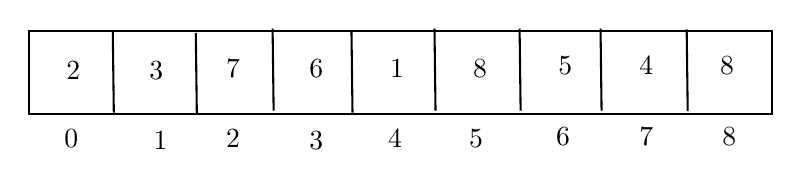
\begin{tikzpicture}[x=0.75pt,y=0.75pt,yscale=-1,xscale=1]
%uncomment if require: \path (0,235); %set diagram left start at 0, and has height of 235

%Shape: Rectangle [id:dp5783048107620253] 
\draw   (160.5,37) -- (518.5,37) -- (518.5,77) -- (160.5,77) -- cycle ;
%Straight Lines [id:da16291536858482958] 
\draw    (278,36) -- (278.5,75.44) ;
%Straight Lines [id:da07147510752614306] 
\draw    (316,37) -- (316.5,76.44) ;
%Straight Lines [id:da7656288099849998] 
\draw    (356,36) -- (356.5,75.44) ;
%Straight Lines [id:da2231965378415679] 
\draw    (397,36) -- (397.5,75.44) ;
%Straight Lines [id:da876762295485208] 
\draw    (436,36) -- (436.5,75.44) ;
%Straight Lines [id:da7355944544210964] 
\draw    (477.5,36.28) -- (478,75.72) ;
%Straight Lines [id:da19422431578327226] 
\draw    (241,38) -- (241.5,77.44) ;
%Straight Lines [id:da5119450193154419] 
\draw    (201,37) -- (201.5,76.44) ;

% Text Node
\draw (497,54) node   [align=left] {8};
% Text Node
\draw (458,54) node   [align=left] {4};
% Text Node
\draw (419,54) node   [align=left] {5};
% Text Node
\draw (378,55) node   [align=left] {8};
% Text Node
\draw (338,55) node   [align=left] {1};
% Text Node
\draw (299,55) node   [align=left] {6};
% Text Node
\draw (259,55) node   [align=left] {7};
% Text Node
\draw (259,89) node   [align=left] {2};
% Text Node
\draw (299,90) node   [align=left] {3};
% Text Node
\draw (337,89) node   [align=left] {4};
% Text Node
\draw (376,89) node   [align=left] {5};
% Text Node
\draw (418,88) node   [align=left] {6};
% Text Node
\draw (458,88) node   [align=left] {7};
% Text Node
\draw (498,88) node   [align=left] {8};
% Text Node
\draw (224,90) node   [align=left] {1};
% Text Node
\draw (181,89) node   [align=left] {0};
% Text Node
\draw (222,56) node   [align=left] {3};
% Text Node
\draw (182,56) node   [align=left] {2};

\end{tikzpicture}
\end{center}

Now, we can translate the array representation to the actual linked list:
\begin{center}
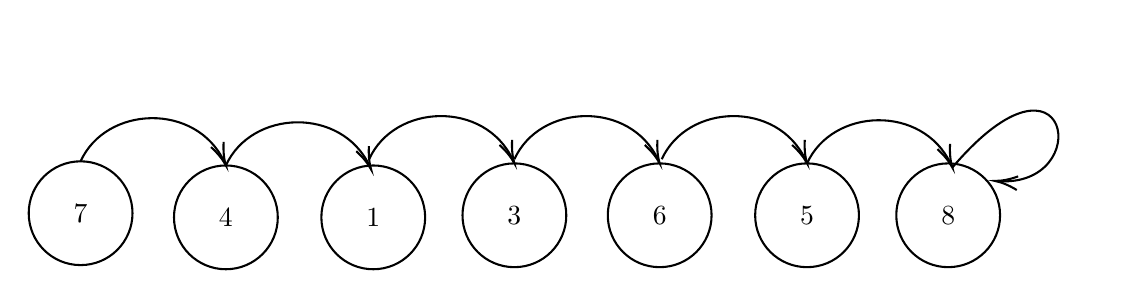
\begin{tikzpicture}[x=0.75pt,y=0.75pt,yscale=-1,xscale=1]
%uncomment if require: \path (0,235); %set diagram left start at 0, and has height of 235
%Shape: Circle [id:dp209412606148338] 
\draw   (26,63) .. controls (26,49.19) and (37.19,38) .. (51,38) .. controls (64.81,38) and (76,49.19) .. (76,63) .. controls (76,76.81) and (64.81,88) .. (51,88) .. controls (37.19,88) and (26,76.81) .. (26,63) -- cycle ;
%Shape: Circle [id:dp8786359500043003] 
\draw   (96,65) .. controls (96,51.19) and (107.19,40) .. (121,40) .. controls (134.81,40) and (146,51.19) .. (146,65) .. controls (146,78.81) and (134.81,90) .. (121,90) .. controls (107.19,90) and (96,78.81) .. (96,65) -- cycle ;
%Shape: Circle [id:dp8199816896544332] 
\draw   (167,65) .. controls (167,51.19) and (178.19,40) .. (192,40) .. controls (205.81,40) and (217,51.19) .. (217,65) .. controls (217,78.81) and (205.81,90) .. (192,90) .. controls (178.19,90) and (167,78.81) .. (167,65) -- cycle ;
%Shape: Circle [id:dp32514518330826625] 
\draw   (305,64) .. controls (305,50.19) and (316.19,39) .. (330,39) .. controls (343.81,39) and (355,50.19) .. (355,64) .. controls (355,77.81) and (343.81,89) .. (330,89) .. controls (316.19,89) and (305,77.81) .. (305,64) -- cycle ;
%Shape: Circle [id:dp9822037867033425] 
\draw   (376,64) .. controls (376,50.19) and (387.19,39) .. (401,39) .. controls (414.81,39) and (426,50.19) .. (426,64) .. controls (426,77.81) and (414.81,89) .. (401,89) .. controls (387.19,89) and (376,77.81) .. (376,64) -- cycle ;
%Shape: Circle [id:dp47504609475506554] 
\draw   (235,64) .. controls (235,50.19) and (246.19,39) .. (260,39) .. controls (273.81,39) and (285,50.19) .. (285,64) .. controls (285,77.81) and (273.81,89) .. (260,89) .. controls (246.19,89) and (235,77.81) .. (235,64) -- cycle ;
%Shape: Circle [id:dp7373998024032005] 
\draw   (444,64) .. controls (444,50.19) and (455.19,39) .. (469,39) .. controls (482.81,39) and (494,50.19) .. (494,64) .. controls (494,77.81) and (482.81,89) .. (469,89) .. controls (455.19,89) and (444,77.81) .. (444,64) -- cycle ;
%Curve Lines [id:da08360307519532739] 
\draw    (51,38) .. controls (63.25,10.99) and (106.71,9.49) .. (120.21,38.2) ;
\draw [shift={(121,40)}, rotate = 247.76] [color={rgb, 255:red, 0; green, 0; blue, 0 }  ][line width=0.75]    (10.93,-3.29) .. controls (6.95,-1.4) and (3.31,-0.3) .. (0,0) .. controls (3.31,0.3) and (6.95,1.4) .. (10.93,3.29)   ;
%Curve Lines [id:da10661682410779472] 
\draw    (121,40) .. controls (133.25,12.99) and (176.71,11.49) .. (190.21,40.2) ;
\draw [shift={(191,42)}, rotate = 247.76] [color={rgb, 255:red, 0; green, 0; blue, 0 }  ][line width=0.75]    (10.93,-3.29) .. controls (6.95,-1.4) and (3.31,-0.3) .. (0,0) .. controls (3.31,0.3) and (6.95,1.4) .. (10.93,3.29)   ;
%Curve Lines [id:da2999819680845789] 
\draw    (190,37) .. controls (202.25,9.99) and (245.71,8.49) .. (259.21,37.2) ;
\draw [shift={(260,39)}, rotate = 247.76] [color={rgb, 255:red, 0; green, 0; blue, 0 }  ][line width=0.75]    (10.93,-3.29) .. controls (6.95,-1.4) and (3.31,-0.3) .. (0,0) .. controls (3.31,0.3) and (6.95,1.4) .. (10.93,3.29)   ;
%Curve Lines [id:da9102701957834004] 
\draw    (260,37) .. controls (272.25,9.99) and (315.71,8.49) .. (329.21,37.2) ;
\draw [shift={(330,39)}, rotate = 247.76] [color={rgb, 255:red, 0; green, 0; blue, 0 }  ][line width=0.75]    (10.93,-3.29) .. controls (6.95,-1.4) and (3.31,-0.3) .. (0,0) .. controls (3.31,0.3) and (6.95,1.4) .. (10.93,3.29)   ;
%Curve Lines [id:da6050891611425984] 
\draw    (331,37) .. controls (343.25,9.99) and (386.71,8.49) .. (400.21,37.2) ;
\draw [shift={(401,39)}, rotate = 247.76] [color={rgb, 255:red, 0; green, 0; blue, 0 }  ][line width=0.75]    (10.93,-3.29) .. controls (6.95,-1.4) and (3.31,-0.3) .. (0,0) .. controls (3.31,0.3) and (6.95,1.4) .. (10.93,3.29)   ;
%Curve Lines [id:da7209329294958705] 
\draw    (401,39) .. controls (413.25,11.99) and (456.71,10.49) .. (470.21,39.2) ;
\draw [shift={(471,41)}, rotate = 247.76] [color={rgb, 255:red, 0; green, 0; blue, 0 }  ][line width=0.75]    (10.93,-3.29) .. controls (6.95,-1.4) and (3.31,-0.3) .. (0,0) .. controls (3.31,0.3) and (6.95,1.4) .. (10.93,3.29)   ;
%Curve Lines [id:da6749246461018108] 
\draw    (471,41) .. controls (527.93,-25.89) and (540.26,50.87) .. (492.95,47.56) ;
\draw [shift={(491.5,47.44)}, rotate = 365.83000000000004] [color={rgb, 255:red, 0; green, 0; blue, 0 }  ][line width=0.75]    (10.93,-3.29) .. controls (6.95,-1.4) and (3.31,-0.3) .. (0,0) .. controls (3.31,0.3) and (6.95,1.4) .. (10.93,3.29)   ;
% Text Node
\draw (469,64) node   [align=left] {8};
% Text Node
\draw (401,64) node   [align=left] {5};
% Text Node
\draw (330,64) node   [align=left] {6};
% Text Node
\draw (260,64) node   [align=left] {3};
% Text Node
\draw (192,65) node   [align=left] {1};
% Text Node
\draw (121,65) node   [align=left] {4};
% Text Node
\draw (51,63) node   [align=left] {7};
\end{tikzpicture}
\end{center}

Then contract the list:

\begin{center}
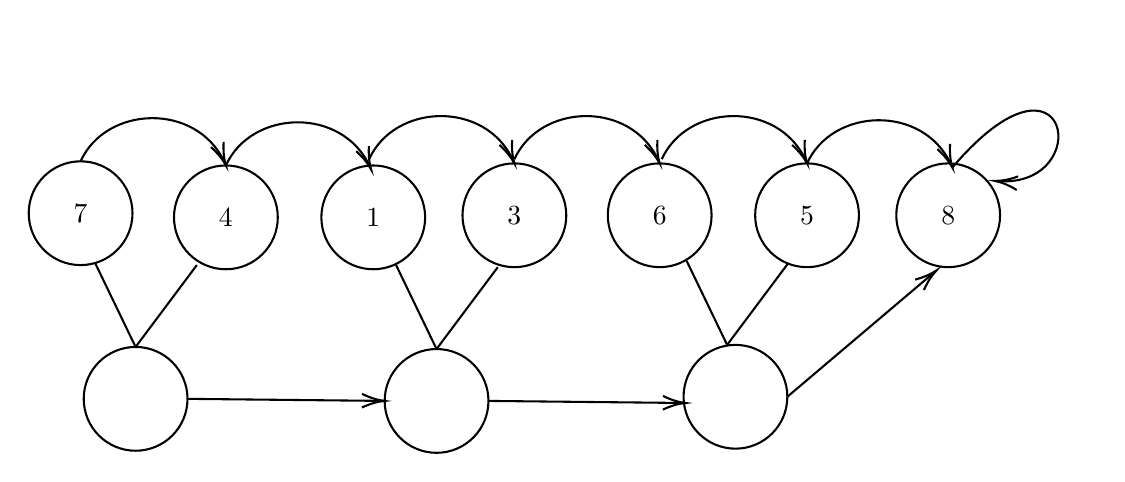
\begin{tikzpicture}[x=0.75pt,y=0.75pt,yscale=-1,xscale=1]
%uncomment if require: \path (0,235); %set diagram left start at 0, and has height of 235

%Shape: Circle [id:dp209412606148338] 
\draw   (26,63) .. controls (26,49.19) and (37.19,38) .. (51,38) .. controls (64.81,38) and (76,49.19) .. (76,63) .. controls (76,76.81) and (64.81,88) .. (51,88) .. controls (37.19,88) and (26,76.81) .. (26,63) -- cycle ;
%Shape: Circle [id:dp8786359500043003] 
\draw   (96,65) .. controls (96,51.19) and (107.19,40) .. (121,40) .. controls (134.81,40) and (146,51.19) .. (146,65) .. controls (146,78.81) and (134.81,90) .. (121,90) .. controls (107.19,90) and (96,78.81) .. (96,65) -- cycle ;
%Shape: Circle [id:dp8199816896544332] 
\draw   (167,65) .. controls (167,51.19) and (178.19,40) .. (192,40) .. controls (205.81,40) and (217,51.19) .. (217,65) .. controls (217,78.81) and (205.81,90) .. (192,90) .. controls (178.19,90) and (167,78.81) .. (167,65) -- cycle ;
%Shape: Circle [id:dp32514518330826625] 
\draw   (305,64) .. controls (305,50.19) and (316.19,39) .. (330,39) .. controls (343.81,39) and (355,50.19) .. (355,64) .. controls (355,77.81) and (343.81,89) .. (330,89) .. controls (316.19,89) and (305,77.81) .. (305,64) -- cycle ;
%Shape: Circle [id:dp9822037867033425] 
\draw   (376,64) .. controls (376,50.19) and (387.19,39) .. (401,39) .. controls (414.81,39) and (426,50.19) .. (426,64) .. controls (426,77.81) and (414.81,89) .. (401,89) .. controls (387.19,89) and (376,77.81) .. (376,64) -- cycle ;
%Shape: Circle [id:dp47504609475506554] 
\draw   (235,64) .. controls (235,50.19) and (246.19,39) .. (260,39) .. controls (273.81,39) and (285,50.19) .. (285,64) .. controls (285,77.81) and (273.81,89) .. (260,89) .. controls (246.19,89) and (235,77.81) .. (235,64) -- cycle ;
%Shape: Circle [id:dp7373998024032005] 
\draw   (444,64) .. controls (444,50.19) and (455.19,39) .. (469,39) .. controls (482.81,39) and (494,50.19) .. (494,64) .. controls (494,77.81) and (482.81,89) .. (469,89) .. controls (455.19,89) and (444,77.81) .. (444,64) -- cycle ;
%Curve Lines [id:da08360307519532739] 
\draw    (51,38) .. controls (63.25,10.99) and (106.71,9.49) .. (120.21,38.2) ;
\draw [shift={(121,40)}, rotate = 247.76] [color={rgb, 255:red, 0; green, 0; blue, 0 }  ][line width=0.75]    (10.93,-3.29) .. controls (6.95,-1.4) and (3.31,-0.3) .. (0,0) .. controls (3.31,0.3) and (6.95,1.4) .. (10.93,3.29)   ;
%Curve Lines [id:da10661682410779472] 
\draw    (121,40) .. controls (133.25,12.99) and (176.71,11.49) .. (190.21,40.2) ;
\draw [shift={(191,42)}, rotate = 247.76] [color={rgb, 255:red, 0; green, 0; blue, 0 }  ][line width=0.75]    (10.93,-3.29) .. controls (6.95,-1.4) and (3.31,-0.3) .. (0,0) .. controls (3.31,0.3) and (6.95,1.4) .. (10.93,3.29)   ;
%Curve Lines [id:da2999819680845789] 
\draw    (190,37) .. controls (202.25,9.99) and (245.71,8.49) .. (259.21,37.2) ;
\draw [shift={(260,39)}, rotate = 247.76] [color={rgb, 255:red, 0; green, 0; blue, 0 }  ][line width=0.75]    (10.93,-3.29) .. controls (6.95,-1.4) and (3.31,-0.3) .. (0,0) .. controls (3.31,0.3) and (6.95,1.4) .. (10.93,3.29)   ;
%Curve Lines [id:da9102701957834004] 
\draw    (260,37) .. controls (272.25,9.99) and (315.71,8.49) .. (329.21,37.2) ;
\draw [shift={(330,39)}, rotate = 247.76] [color={rgb, 255:red, 0; green, 0; blue, 0 }  ][line width=0.75]    (10.93,-3.29) .. controls (6.95,-1.4) and (3.31,-0.3) .. (0,0) .. controls (3.31,0.3) and (6.95,1.4) .. (10.93,3.29)   ;
%Curve Lines [id:da6050891611425984] 
\draw    (331,37) .. controls (343.25,9.99) and (386.71,8.49) .. (400.21,37.2) ;
\draw [shift={(401,39)}, rotate = 247.76] [color={rgb, 255:red, 0; green, 0; blue, 0 }  ][line width=0.75]    (10.93,-3.29) .. controls (6.95,-1.4) and (3.31,-0.3) .. (0,0) .. controls (3.31,0.3) and (6.95,1.4) .. (10.93,3.29)   ;
%Curve Lines [id:da7209329294958705] 
\draw    (401,39) .. controls (413.25,11.99) and (456.71,10.49) .. (470.21,39.2) ;
\draw [shift={(471,41)}, rotate = 247.76] [color={rgb, 255:red, 0; green, 0; blue, 0 }  ][line width=0.75]    (10.93,-3.29) .. controls (6.95,-1.4) and (3.31,-0.3) .. (0,0) .. controls (3.31,0.3) and (6.95,1.4) .. (10.93,3.29)   ;
%Curve Lines [id:da6749246461018108] 
\draw    (471,41) .. controls (527.93,-25.89) and (540.26,50.87) .. (492.95,47.56) ;
\draw [shift={(491.5,47.44)}, rotate = 365.83000000000004] [color={rgb, 255:red, 0; green, 0; blue, 0 }  ][line width=0.75]    (10.93,-3.29) .. controls (6.95,-1.4) and (3.31,-0.3) .. (0,0) .. controls (3.31,0.3) and (6.95,1.4) .. (10.93,3.29)   ;
%Straight Lines [id:da09021454387424288] 
\draw    (58,87) -- (77.5,127.44) ;
%Straight Lines [id:da1433127111995599] 
\draw    (107,88) -- (77.5,127.44) ;
%Straight Lines [id:da6502066819956911] 
\draw    (203,88) -- (222.5,128.44) ;
%Straight Lines [id:da22056480876502604] 
\draw    (252,89) -- (222.5,128.44) ;
%Straight Lines [id:da20473545330807807] 
\draw    (343,86) -- (362.5,126.44) ;
%Straight Lines [id:da18676136219017514] 
\draw    (392,87) -- (362.5,126.44) ;
%Shape: Circle [id:dp6410138198386195] 
\draw   (52.5,152.44) .. controls (52.5,138.63) and (63.69,127.44) .. (77.5,127.44) .. controls (91.31,127.44) and (102.5,138.63) .. (102.5,152.44) .. controls (102.5,166.24) and (91.31,177.44) .. (77.5,177.44) .. controls (63.69,177.44) and (52.5,166.24) .. (52.5,152.44) -- cycle ;
%Shape: Circle [id:dp843236816358602] 
\draw   (197.5,153.44) .. controls (197.5,139.63) and (208.69,128.44) .. (222.5,128.44) .. controls (236.31,128.44) and (247.5,139.63) .. (247.5,153.44) .. controls (247.5,167.24) and (236.31,178.44) .. (222.5,178.44) .. controls (208.69,178.44) and (197.5,167.24) .. (197.5,153.44) -- cycle ;
%Shape: Circle [id:dp49741461298780953] 
\draw   (341.5,151.44) .. controls (341.5,137.63) and (352.69,126.44) .. (366.5,126.44) .. controls (380.31,126.44) and (391.5,137.63) .. (391.5,151.44) .. controls (391.5,165.24) and (380.31,176.44) .. (366.5,176.44) .. controls (352.69,176.44) and (341.5,165.24) .. (341.5,151.44) -- cycle ;
%Straight Lines [id:da3260528284556792] 
\draw    (102.5,152.44) -- (195.5,153.42) ;
\draw [shift={(197.5,153.44)}, rotate = 180.6] [color={rgb, 255:red, 0; green, 0; blue, 0 }  ][line width=0.75]    (10.93,-3.29) .. controls (6.95,-1.4) and (3.31,-0.3) .. (0,0) .. controls (3.31,0.3) and (6.95,1.4) .. (10.93,3.29)   ;
%Straight Lines [id:da8703932924324034] 
\draw    (247.5,153.44) -- (340.5,154.42) ;
\draw [shift={(342.5,154.44)}, rotate = 180.6] [color={rgb, 255:red, 0; green, 0; blue, 0 }  ][line width=0.75]    (10.93,-3.29) .. controls (6.95,-1.4) and (3.31,-0.3) .. (0,0) .. controls (3.31,0.3) and (6.95,1.4) .. (10.93,3.29)   ;
%Straight Lines [id:da6262153714243609] 
\draw    (391.5,151.44) -- (461.97,91.73) ;
\draw [shift={(463.5,90.44)}, rotate = 499.73] [color={rgb, 255:red, 0; green, 0; blue, 0 }  ][line width=0.75]    (10.93,-3.29) .. controls (6.95,-1.4) and (3.31,-0.3) .. (0,0) .. controls (3.31,0.3) and (6.95,1.4) .. (10.93,3.29)   ;

% Text Node
\draw (469,64) node   [align=left] {8};
% Text Node
\draw (401,64) node   [align=left] {5};
% Text Node
\draw (330,64) node   [align=left] {6};
% Text Node
\draw (260,64) node   [align=left] {3};
% Text Node
\draw (192,65) node   [align=left] {1};
% Text Node
\draw (121,65) node   [align=left] {4};
% Text Node
\draw (51,63) node   [align=left] {7};
\end{tikzpicture}
\end{center}

\subsection{Quick Sort}
\textsc{QuickSort} is naturally very parallel as we can use the \textsc{Filter} function when splitting the elements with the pivot which is parallel.

\subsection{Merge Sort}
Is \textsc{MergeSort} parallel? 
Say if we halve an array
$$\{\underbrace{...}_{n/2}\underbrace{...}_{n/2}\}$$
then, the span of our \textsc{MergeSort} will be:
$$S(n) = S(n/2) + S_{\text{merge}}$$
The question is, how fast can we merge two arrays? We first try to create another function $\textsc{Kth}(k,A,B)$ to help us merging.
\begin{claim}
	Given 2 sorted sequence $A$ and $B$, there is a function, $\textsc{Kth}(k,A,B)$, that returns $l_A,l_B, l_A +l_B = k$ such that $A[:l_A]$ and $B[:l_B]$ are the smallest $k$ elements, of A+B done in $O(|A|+|B|)$ work, $O(\log^2{(|A|+|B|))} $ span.
\end{claim}
The implementation of this is given in the review paper. With the \textsc{Kth} function, we can now fo merge easily.
\begin{algorithm}[H]
	\caption{Parallel Merge}
	\begin{algorithmic}[1]
		\Function{Merge}{A, B}
		\If {$len(A) =0$}
		\State \Return $B$
		\EndIf
		\If {$len(B) =0$}
		\State \Return $A$
		\EndIf
		\State {$m \gets(len(A)+len(B))/2$ }
		\State {$la,lb \gets \textsc{Kth}(m, A,B)$}
		\State {$A',B' = \textsc{Merge}(A[:la],B[:lb]) \parallel \textsc{Merge}(A[la:],B[lb:])$}
		\State \Return {$A' + B'$}
		\EndFunction
	\end{algorithmic}
\end{algorithm}

The work done for \textsc{Merge} above is $$W(n) = W(n/2) + W(n-n/2) + O(\log{n})$$
which solves to $O(n)$ where $n = |A| + |B|$, and the span is given by
$$S(n) = S(n/2) + O(\log{n})$$
which solves to $O(\log^2n)$\\

Now that, the span of \textsc{Merge} is $O(log^2n)$, we can go back to \textsc{MergeSort} span analysis to see that the span of \textsc{MergeSort} can be expressed to 
$$S(n) = S(n/2) + O(\log^2n)$$
which solves to $O(\log^3n)$.

\end{document}
